%%%%%% CMB-S4 Simulations and Data Analysis Chapter, Forecasting Section  %%%%%%%%%%%%%%%%

\section{Forecasting}

Here we describe the main approaches used by our community for forecasting the expected performance of CMB-S4. For assessing the expected performance for large-scale B-modes, two central considerations are Galactic foregrounds and ability to delens the data, as well as a realistic assessment of instrument noise at large scales. 

To assess the science return from the smaller-scale polarization two-point functions (TE,EE), and from the lensing four-point function ($\kappa \kappa$), extragalactic foregrounds and instrumental noise are the key considerations.

To forecast the return of the thermal Sunyaev-Zel'dovich effects, an estimate of the expected cluster counts as a function of mass and redshift is the core statistic, combined with an estimate of how well the masses can be calibrated using overlaps with weak lensing surveys. For the kinetic Sunyaev-Zeldovich effect, extragalactic foregrounds and overlap with spectroscopic surveys must all be considered. 

\begin{figure}[htbp]
\centering
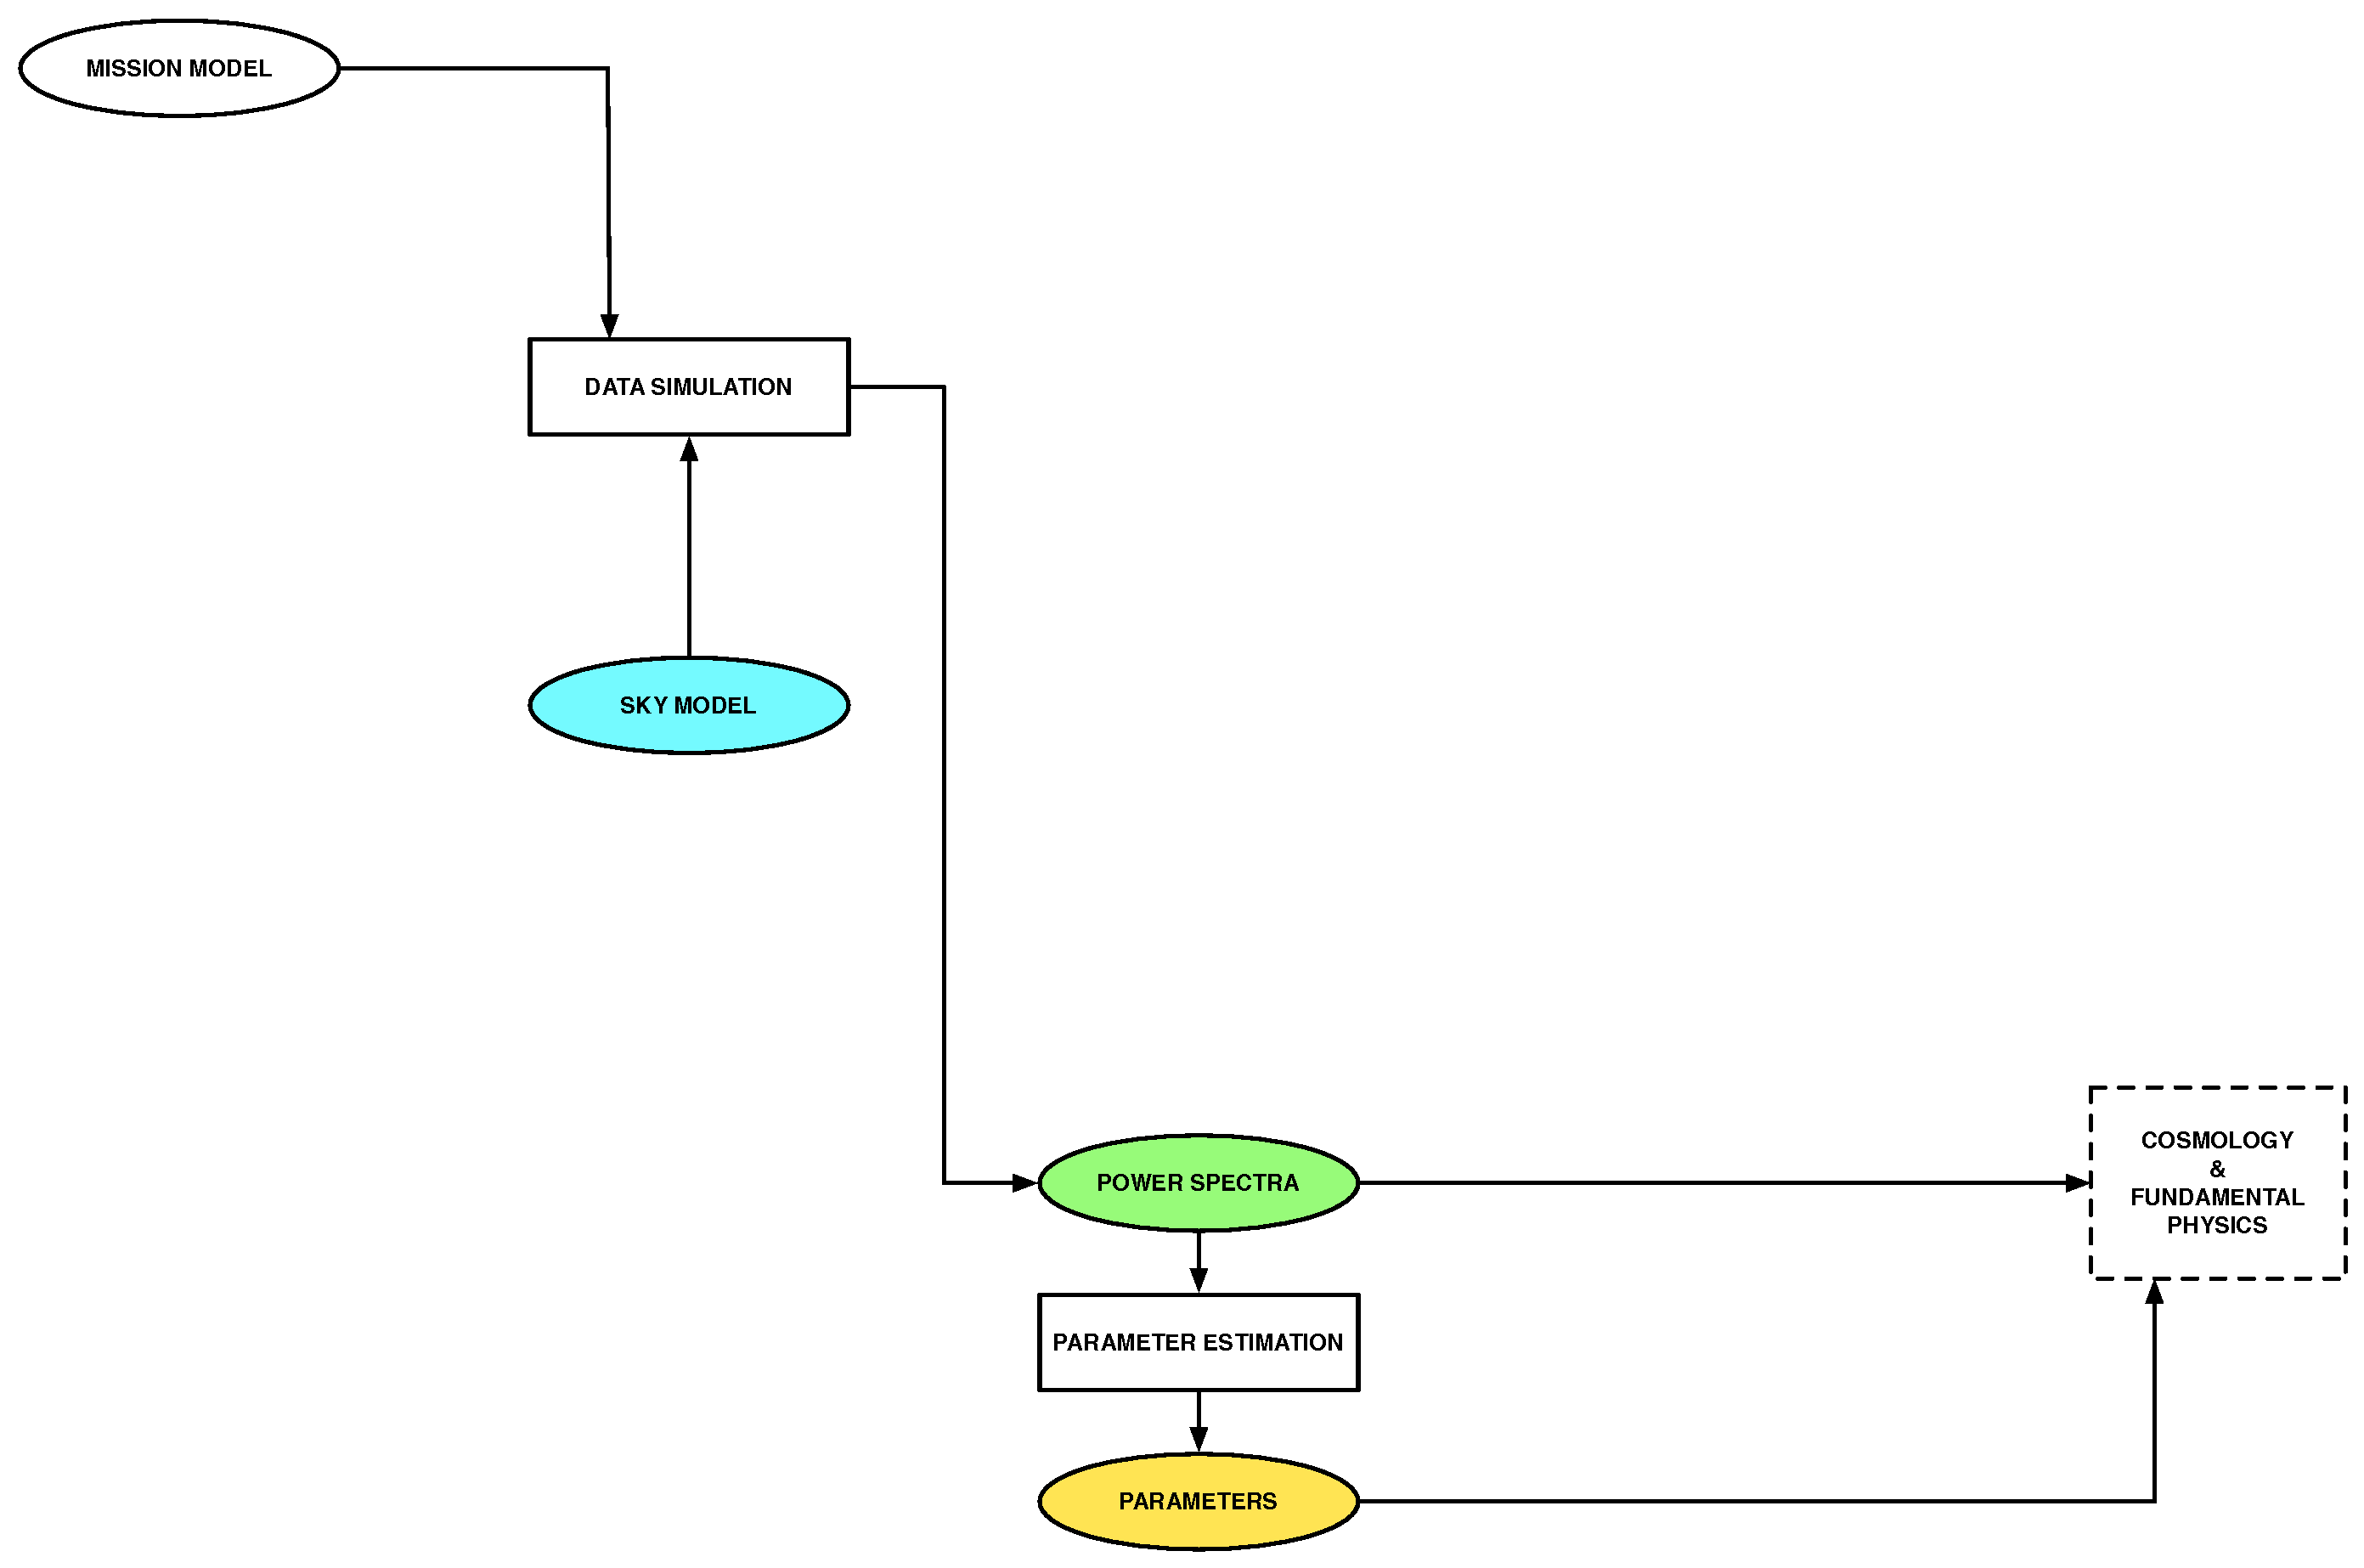
\includegraphics[width=1\textwidth]{Analysis/fc}
\caption{The forecasting subset of the CMB simulation and data analysis pipeline}
\label{default}
\end{figure}


\subsection{Limits on the tensor-to-scalar ratio}

\subsubsection{Spectrum-based domain forecasting}
{\bf Forecasting in spectral domain coming from John Kovac}

\subsubsection{Map-based domain forecasting}

Foregrounds are intrinsically non-Gaussian, so it is beneficial to consider approaches directly in map space, to check the robustness of spectrum-based approaches, in particular in the case of pessimistic foregrounds where the spectral indices or dust emissivities have spatial variation. Here one of the approaches our community uses is a Bayesian model fitting method.

Maps of the CMB plus Galactic foreground sky and instrument noise are simulated at each of the CMB-S4 frequencies and integrated across the expected bandpass, using Galactic models as described for example in Section \ref{sec:models}. A parameterized model is then fit to the simulated maps, for example fitting the CMB, thermal dust, and synchrotron in small pixels, and typically the synchrotron spectral index and dust emissivity and temperature in larger pixels of order degree-scale. The BB power spectrum of the foreground-marginalized CMB map is then estimated, and convered into an estimate of r and its uncertainty. Our community has at least three such codes.

This method allows for an assessment of the expected bias on $r$ if the model does not match the simulation, and shows how much the expected uncertainty on $r$ would increase if more complicated foreground models are explored \citep[e.g. as in,][]{armitage-caplan/etal:2011,ramazeilles/etal:2015}. It is more computationally expensive than spectral-domain forecasts though, so we use this approach on a smaller-subset of explorations. 

\subsection{Limits on parameters from TT/TE/EE/$\kappa\kappa$}

{\bf Jo writing - much of this currently copied from Allison et al, in process of cutting and editing}

To forecast the expected constraints on cosmological parameters for CMB-S4, many of our community's codes use a Fisher matrix method, combining S4 specifications with other available datasets, for example the data from Planck and expected measurements of Baryon Acoustic Oscillations and other low redshift data. 

For the noise levels of Planck, we assume that a data release including reliable polarization data will have happened, and forecast results that include TE and EE data and also large-scale polarization from HFI. This follows approaches in e.g. \cite{allison/etal:2015}.

We assume uniform priors on all parameters, and evaluate the Fisher matrix at fiducial parameters. To compute the Fisher matrix we use the CMB power spectra, and also add BAO distance measurements. For the CMB, we use the lensed power spectrum between each pair of fields $X, Y$ from their spherical harmonic coefficients:
%
\begin{equation}
\label{eqEstimator}
\hat{C}^{XY}_\ell = \frac{1}{2\ell+1}\sum_{m=-\ell}^{m=\ell} x^{*}_{\ell m} y_{\ell m}.
\end{equation}
%
The estimated power spectrum follows a Gaussian distribution to good approximation at small scales. For a full-sky survey, we have 
%
\begin{equation}
-2\ln\mathcal{L}(\boldsymbol{\theta}) = -2\sum_\ell \ln p( \hat{C}_\ell | \boldsymbol{\theta}) \\
=  \sum_\ell  \Big[ (\hat{C}_\ell - C_\ell(\boldsymbol{\theta}) )^\top  \mathbb{C}^{-1}_\ell(\boldsymbol{\theta}) \big(\hat{C}_\ell - C_\ell(\boldsymbol{\theta})) + \ln \det(2 \pi \mathbb{C}_\ell(\boldsymbol{\theta})) \Big]
\end{equation}
%
where $ \hat{C}_\ell = (\hat{C}_\ell^{TT}, \hat{C}_\ell^{TE}, ...) $ contains auto- and cross-spectra and $\mathbb{C}_\ell$ is their covariance matrix. Inserting this likelihood into Eq.~\ref{eqFisher} and neglecting parameter dependence in the power spectrum covariance matrix one obtains
%
\begin{equation}
F_{ij} = \sum_\ell \frac{\partial C^\top_l}{\partial \theta_i} \mathbb{C}^{-1}_\ell \frac{\partial C_l}{\partial \theta_j}.
\end{equation}
%
From Eq.~\ref{eqEstimator}, and applying Wick's theorem, the covariance matrix for the power spectra has elements
%
\begin{equation}
\mathbb{C}(\hat{C}_l^{\alpha \beta}, \hat{C}_l^{\gamma \delta}) = \frac{1}{(2l+1)f_{\rm sky}} \big[ (C_l^{\alpha \gamma} + N_l^{\alpha \gamma}) (C_l^{\beta \delta} + N_l^{\beta \delta})  \\
+ (C_l^{\alpha \delta} + N_l^{\alpha \delta}) (C_l^{\beta \gamma} + N_l^{\beta \gamma}) \big],
\end{equation}
%
where $\alpha, \beta, \gamma, \delta \in \{T, E, B, \kappa_c\}$ and $f_{\rm sky}$ accounts for the loss of information due to partial sky coverage \cite{Hobson:1996,dePutter:2009}. 
%, 


\subsubsection{Instrument noise}
Noise spectra are generated for each observable assuming the sum of white noise and atmospheric noise:
%
\begin{equation}
N^{\alpha \alpha}_\ell = (\Delta T)^2 \exp \left( \frac{\ell(\ell + 1) \theta^2_{\rm FWHM}}{8 \ln 2} \right)
\end{equation}
%
for $\alpha \in \{T, E, B\}$, where $\Delta T$ ($\Delta P$ for polarization) is the map sensitivity in $\mu$K-arcmin and $\theta_{\rm FWHM}$ is the beam width. 

To estimate the atmospheric noise level, we consider levels at the South Pole and in Chile.
For polarization our nominal estimate is white noise, assuming half wave plates.

%
The CMB lensing reconstruction noise is calculated using the \cite{Hu:2002} quadratic-estimator formalism. We neglect non-Gaussian terms in the power spectrum covariance, and also neglect the BB spectrum as it does not contribute significantly to upcoming constraints and has a highly non-Gaussian covariance \cite{Benoit-Levy:2012}. 

When relevant, we can also add information from Baryon Acoustic Oscillation (BAO) experiments by computing the BAO Fisher matrix:
%
\begin{equation}
F_{ij}^{\rm BAO} = \sum_{k} \frac{1}{\sigma_{f,k}^2}\frac{\partial f_k}{\partial \theta_i}\frac{\partial f_k}{\partial \theta_j}
\end{equation}
%
where $f_k \equiv f(z_k) = r_s/d_V(z_k)$ is the sound horizon at photon-baryon decoupling $r_s$ over the volume distance $d_V$ to the source galaxies at redshift $z_k$. These real and forecast data are reported in Table \ref{tabBAO}.

The total Fisher information matrix is given by the sum of the CMB and BAO Fisher matrices, and is inverted to forecast parameter covariances.  An alternative MCMC approach using simulated data can be taken to account for non-Gaussianity of the posterior \cite[e.g.,][]{Hall:2012}, but the Gaussian approximation is likely increasingly good as the data quality improve from {\sl Planck} through S3 to S4. 

For the CMB power spectra, we set a maximum multipole for the recoverable information $\ell^T_{\rm max} = 3000$, $\ell^P_{\rm max} = 4000$ for the future S3 and S4 experiments, as foregrounds are expected to be limiting at smaller scales. We also set a minimum multipole due to the challenge of recovering large-scales from the ground, and consider two options for S4, $\ell=50$ and $\ell=5$. We include Planck data at the scales $\ell<\ell_{\rm min}$. 

We also consider the lensed TT, TE, EE, BB spectra, rather than the unlensed fields and convergence.




\subsection{Limits on parameters from tSZ/kSZ}
